\articlehead{My Little MLP Adventure: Verdict}{JM}{2013}

I don't normally watch children's cartoons.

Yet I sat down and watched several hours of \textit{My Little Pony}, in an attempt to understand why it has become so visible within the furry community. Here is what I discovered.

I learned that \textit{My Little Pony} is a cartoon aimed at an audience of young girls. It's very well made: high production values, good animation, talented voice acting, robust and logical stories. That's basically all it is.

Except that it has gained a huge adult following, including a high proportion of furries. The adult fans are largely male, young, and geeky; a demographic that not coincidentally describes a big swathe of the furry population.

I asked a few pony lovers why \textit{MLP} is so popular. I received responses like \textit{`the brony community is great'}; or, \textit{`because \textit{MLP} has critical mass online, so you can't avoid it'}; or, \textit{`because it's so childish that people like to make fun of it'}. All of these arguments may be true but they require there to be a large pre-existing \textit{MLP} audience: none of them explain why so many people started -- and kept -- watching and caring in the first place.

The appeal of \textit{MLP} can be inferred by looking at its audience: girls, and young geeky men (with some exceptions). \textit{MLP} is a big deal because its art style and subject matter make it easy for people to identify with the characters. \textit{MLP} appeals to people who are developing empathy.

Allow me to explain.

\subsection*{1. They Have Big Eyes}

The ponies have big eyes: big, big eyes. Their heads are the size of their bodies; their eyes take up half their heads.

We humans are social beings. Most of our communication takes place through body language, especially facial expressions. We see faces in inanimate objects all the time: in sand dunes on Mars, or a slice of toast.

\begin{figure}
  \begin{center}
    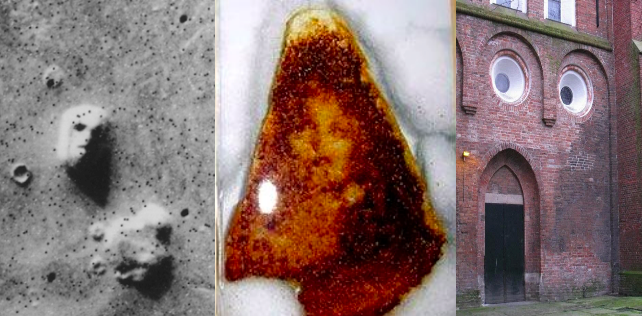
\includegraphics[width=\textwidth]{content/assets/mlp--faces}
  \end{center}
  \caption{Faces in inanimate objects: sand dunes on mars; the Virgin Mary on toast; a building.}
\end{figure}

The ability to infer human faces from little visual information is an evolved human trait, akin to the way zebras identify close family members by stripe patterns.

Eyes are especially important. For example, disembodied pictures of eyes, presented with no context, have been shown to have significant effects on behaviour. One study showed that pictures of eyes caused people to triple their voluntary donation for a cup of coffee, compared with pictures of flowers (ref); another found that posters of eyes in a cafeteria halved littering incidents, compared with pictures of flowers (ref).

\begin{figure}
  \begin{center}
    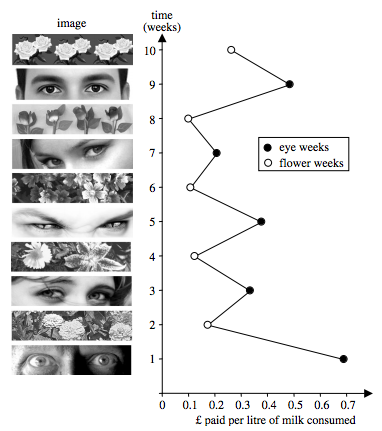
\includegraphics{content/assets/mlp--eyes}
  \end{center}
  \caption{Eyes.}
\end{figure}

Service industry workers relying on tips would be well advised to sketch a smiley face on each customer's bill.

The ponies have huge eyes, and these eyes make it clear what they are thinking. This is narratively elegant -- we don't need everything spelt out -- and it makes us feel like we understand the pony. This is empathy, and it's why \textit{MLP} is so engaging. Cartoons in general provoke a similar feeling, but \textit{MLP} is more effective due to the huge, expressive, well animated, and well directed eyes.

It helps that the characters are female too, because…

\subsection*{2. The Idea of `Masculinity' is Kinda Dumb}

The gender of the ponies is relevant, especially for the original target audience. Girls watching \textit{MLP} can identify with the characters, and engage in play as an imaginary participant in the pony universe.

It's also relevant for the unintended audience -- the young men -- because of the state of masculinity in the 21st century. To be masculine, traditionally, was to be a force of change of the world, to be a creator. This has changed, and being masculine is now about being a detached observer of society, a trait that correlates with cynicism, sarcasm, and snarkiness. This can be (and often is) intelligent and worthwhile, but it's not healthy. It creates a world where men are driven away from participation, because participation can lead to failure, and failure breaks the detached observer facade. (The only other option is to be a flawless hero, fine for cartoons.)

The female characters of \textit{MLP} can explore friendship and creation without a requirement to be heroic or detached: they can `have adventures' and succeed or fail on their own terms. A male version of \textit{MLP} couldn't do that, and still ring true.

As an aside, it's nice to see that the gender of the characters isn't relevant to the male viewership. Women are simply portrayed as the norm in the context of the pony universe, and that's okay.

So beyond its core audience, \textit{MLP} attracts…

\subsection*{3. Geeks with High IQs}

People with maturing social skills may find empathetic experiences to be rare. This is common among intelligent male geeks because:

\begin{itemize}
  \item Men tend to mature socially more slowly than women.
  \item Geeks may use their intelligence as a crutch to manage social situations, relying on their analytical skills rather than their developing emotional skills.
\end{itemize}

Such geeks may prefer to socialize where interpretation of subtle body language is less important: perhaps online, or otherwise where behaviour is constrained by rules (stereotypically over a game of Dungeons \& Dragons or Magic: The Gathering).

People with limited empathic skills will often find social situations to be stressful and exhausting. If you are relying on an analytical brain in a social situation (rather than an empathic brain), it requires a lot of concentration, especially if there are more than a few people present. Geeks often find socializing stressful, and will sometimes incorrectly misdiagnose themselves as being introverted, or having mild autism. They're not: they are just lower in empathy than most people, something that will grow given time.

\secdiv

\textit{\textit{My Little Pony}}, then, is going to meet an unconscious emotional need for many young men: the need for empathy. Young and geeky men will tend to find \textit{MLP} very engaging, as they will be able to easily understand and empathize with the characters.

And if some of the fans are geeky, a subset of them are going to hyperfocus on the show, like Trekkies or any other geeky fandom. These hyperfocussed geeks make up \textit{MLP}'s committed and intense following of bronies.

For the rest for us, \textit{MLP} is engaging and easy to follow. We can `see' what is going on inside the heads of the main characters -- eyes being the windows of the soul -- so the show is pleasing and familiar. It's a relaxing viewing experience, almost hypnotic. As an experiment, my fellow viewers and I watched for a while with no sound, and we were able to follow the story with no apparent loss of fidelity.

For all its value, \textit{MLP} is not high art. The humour is childish slapstick, a pre-teen version of Ow My Balls. The characters are simply drawn and simply motivated. The morals of the show are relentlessly, mind-numbingly positive. As an adjunct to our no-sound experiment, we also tried looking away so we were only exposed to the soundtrack: the script, the songs, and the foley artistry are nauseating, pandering, moronic. Like America's Funniest Home Videos without the videos, but less fun.

Even with its limitations, the resonance of \textit{MLP} with many members of the furry community is genuine and valuable. I suspect that its influence on furry culture will grow: like The Lion King or Robin Hood, \textit{MLP} will be a gateway to furry for many people. The \textit{MLP} fandom is innately limited by its subject, and many pony-fans will find the furry community to be an environment that allows them to grow beyond the constraints of the \textit{MLP} universe. Pony lovers will easily fit into the furry world, a world which allows them to explore their connection with anthropomorphic animals on their own terms. As I've written in previous articles for [adjective][species], furry is a community that can help personal growth and maturation.

Such opportunities for personal growth will be greatest for younger \textit{MLP} fans. Typically, people reach emotional maturity at about age 30, although this isn't a hard limit.

I would argue that older fandom geeks, and they exist in any fandom, are limited people. They have failed to develop broader emotional skills that would allow them to look outside of their own interests and into the wider world. Such people limit their intake of culture to a small number of simple artefacts (\textit{MLP}, Star Trek, whathaveyou) and are prone to hyperfocus on the minutiae of that culture. This doesn't make them bad -- such people are often great servants to their fandom -- but they tend not to be well-rounded people.

There are broader horizons out there. Most geeky young men will fit the stereotype of the high school nerd who turns out to be the hunk at the 15-year reunion. Geeky young men remain intelligent and capable human beings, gaining empathetic skills later in life. They grow and shed their social awkwardness, learning to fit in without compromising their identity. The `sexy geek' is a well known phenomenon, to the point that fashion houses try to package and sell the `geek chic' formula. More simply, furries can take a look around and observe that the older members of the group are often confident, happy, and sexy.

Furry provides an environment for such growth. We're diverse. We can engage with cultures like \textit{MLP} without being defined by them. We can equally decide that \textit{MLP} isn't relevant to our personal interests and look elsewhere. This is what's great about our community: we create our own culture. Many \textit{MLP} fans will discover furry over the coming years, and learn such joys.
